\appendix
\section{Additional Metrics and Condition Definitions}
\label{app:conditions}
Core uses pseudonyms, procedural questions, and disconnected distractors unless specified. K1 is source-card triples; K2 adds adjacent distractors; K3 hosts triples on destination cards; K4 repeats them on both endpoint cards. K5 is templated text; K6 is its adjacent variant. K7/K8 use direct queries with triples/text. K5k expresses links through matching attribute values. R1-matched/R2-matched use real names with disconnected/adjacent triples. R0/K0 retain names/types only. Their prompt permits prior name knowledge and requests an insufficient-evidence flag; other controlled conditions restrict evidence to supplied cards.

Fact-preserving pairs retain designated unique relations and targets. Noise pairs retain the question/reference while altering distractor context. A change in presentation may still alter repetition, salience, and token length. Native metadata is not assumed sufficient for every graph-defined target.

\subsection{Controlled Core Profiles}
\label{app:coreprofiles}
\begin{figure*}[t]
\centering
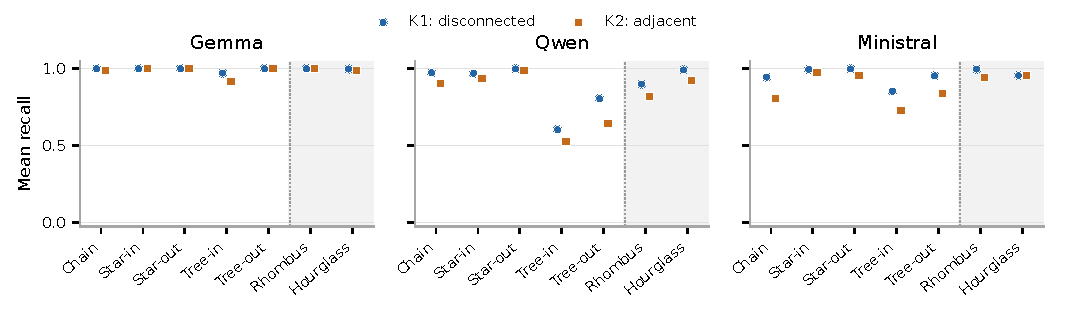
\includegraphics[width=\textwidth]{figures/recall_motifs.pdf}
\caption{Core recall with explicit source-card relations: K1 disconnected and K2 adjacent distractors, 100 planned tasks per point. The first five families have six nodes; shaded rhombus/hourglass use four/five and are not equal-size contrasts. Invalid outcomes contribute zero. These are descriptive macro means, without inferential error bars.}
\Description{Recall across seven graph-pattern families for three models. Incoming-tree recall is below outward-star recall, with model-dependent changes under adjacent contexts.}
\label{fig:motifs}
\end{figure*}

Figure~\ref{fig:motifs} shows task-family differences, including five families at the common six-node reference size. Under K1, six-node incoming-tree recall is 0.972 for Gemma, 0.603 for Qwen, and 0.853 for Ministral. Outward stars are close to complete coverage. The common size does not eliminate differences in query semantics, relation types, or sampled entities; it rules out a node-count-only description of these observed task profiles, not every competing explanation.

Precision supplies a different view. Qwen's K1 incoming-tree precision is 0.988, despite recall of 0.603 and exact recovery of 0.150. It often selects a small, mostly reference-consistent set while failing to cover the reference. Gemma's corresponding precision is 1.000 and exact 0.870. Appendix~\ref{app:conditions} reports precision profiles separately rather than combining the two quantities into one F1 curve.

\begin{figure*}[t]
\centering
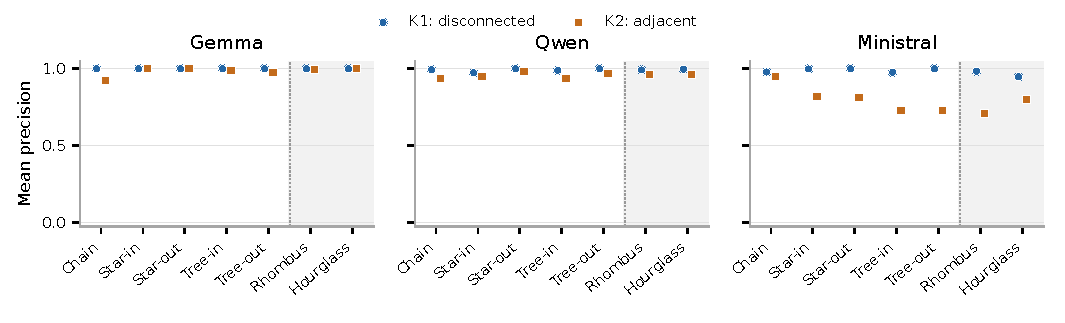
\includegraphics[width=\textwidth]{figures/precision_motifs.pdf}
\caption{Precision companion to Figure~\ref{fig:motifs}: Core K1/K2, 100 planned tasks per point, invalid zero. Shaded families have different sizes. High precision can coexist with incomplete coverage; this is a descriptive saved-score profile without confidence intervals.}
\Description{Precision across graph families, with near-ceiling disconnected scores for many cells and lower precision for several Ministral adjacent conditions.}
\label{fig:precisionmotifs}
\end{figure*}
\begin{figure*}[t]
\centering
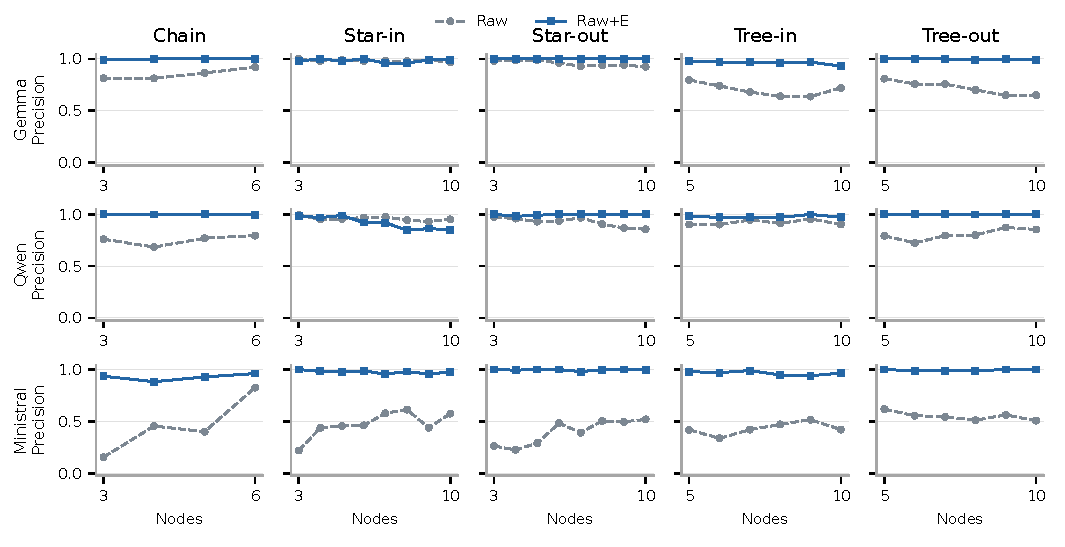
\includegraphics[width=\textwidth]{figures/precision_sizes.pdf}
\caption{Precision companion to Figure~\ref{fig:sizes}, retaining all three models and five variable-size families under Raw/Raw+E. Each point has 100 planned tasks; invalid contributes zero. Size cohorts differ and no curve is interpreted as a causal graph expansion.}
\Description{Precision over subgraph size. Explicit-overlay precision often remains high even where corresponding recall is incomplete.}
\label{fig:precisionsizes}
\end{figure*}

\begin{table}[t]
\caption{All Core condition means: recall, with 700 planned outcomes per model/condition and invalid zero. These are descriptive macro means.}
\label{tab:coreall}
\centering\small
\begin{tabular}{lrrr}
\toprule
Condition & Gemma & Qwen & Ministral \\
\midrule
K0 & 0.182 & 0.189 & 0.299 \\
K1 & 0.996 & 0.892 & 0.957 \\
K2 & 0.985 & 0.820 & 0.885 \\
K3 & 0.996 & 0.896 & 0.914 \\
K4 & 0.993 & 0.951 & 0.950 \\
K5 & 0.993 & 0.857 & 0.956 \\
K6 & 0.979 & 0.794 & 0.911 \\
K7 & 0.996 & 0.888 & 0.941 \\
K8 & 0.990 & 0.853 & 0.939 \\
K5k & 0.988 & 0.850 & 0.918 \\
R0 & 0.322 & 0.282 & 0.298 \\
R1-matched & 0.985 & 0.817 & 0.844 \\
R2-matched & 0.973 & 0.750 & 0.762 \\
\bottomrule
\end{tabular}

\end{table}
\begin{table}[t]
\caption{Precision counterpart to Table~\ref{tab:coreall}, using the same planned populations and failure policy.}
\label{tab:coreprecision}
\centering\small
\begin{tabular}{lrrr}
\toprule
Condition & Gemma & Qwen & Ministral \\
\midrule
K0 & 0.994 & 0.974 & 0.130 \\
K1 & 1.000 & 0.992 & 0.983 \\
K2 & 0.983 & 0.957 & 0.791 \\
K3 & 0.999 & 0.992 & 0.976 \\
K4 & 0.996 & 0.996 & 0.950 \\
K5 & 0.999 & 0.992 & 0.980 \\
K6 & 0.974 & 0.958 & 0.751 \\
K7 & 1.000 & 0.989 & 0.971 \\
K8 & 1.000 & 0.993 & 0.991 \\
K5k & 0.996 & 0.987 & 0.965 \\
R0 & 0.936 & 0.861 & 0.391 \\
R1-matched & 0.991 & 0.992 & 0.979 \\
R2-matched & 0.984 & 0.958 & 0.838 \\
\bottomrule
\end{tabular}

\end{table}

\paragraph{Output signatures and diagnostic limits.}
An exact one-hop signature means the saved selection equals the anchor plus all permitted first-hop neighbours. On the inspected Qwen K1 six-node incoming-tree tasks, this occurs in 71/100 outputs; K3/K4/K7 have 76/31/52. Their exact-reference counts are 16/51/16, compared with 15 in K1. This distinguishes elimination of a signature from correction of the task. All these Qwen cells have 100 valid outcomes. The same original 71 one-hop outputs become exact on 13 K3, 38 K4, and ten K7 tasks. Under K4, six initially exact outputs lose exactness. No new interval or significance test is attached to these post-hoc contrasts.

Ministral has 15/100 initial one-hop sets and 54/100 exact outputs in K1. K4 makes eight of those one-hop sets exact and loses exactness on nine initially exact tasks; total exact recovery is 62/100. Gemma's aggregate scores remain in all main tables/figures, but the archive lacks identities for this finer check. Output signatures do not prove hidden search depth or branch order.

On the inspected Qwen K1 incoming-tree inputs, undirected depth-two and directed depth-three coverage agree with the correct reference on all 100 tasks. Under K2 these alternative targets differ on 97/100 and 10/100 tasks, respectively; no Qwen output exactly matches those distinct alternative sets. This does not rule out mixed or partial rule violations. This slice has no terminal-type stopping condition, so it cannot diagnose terminal-type errors.

\paragraph{Analytical and uncertainty context.}
Select-all has recall one on every nonempty reference by definition, and precision equal to the reference proportion in the 25-candidate pool. These are analytical reference rules, not executed LLM/retrieval baselines. A full connected-component baseline was not computed. Earlier archive uncertainty analyses cover F1/exact with anchor-conditional assumptions; no such bands are reused for the present recall/precision results. Original exact scores, earlier metrics, native/legacy panels, and incomplete incremental histories remain in the supporting source artifacts rather than being pooled into the main populations.

\section{Author-Supplied Cypher Extraction Specification}
\label{app:cypher}
The following Cypher query was supplied by the authors for the appendix. Whitespace is normalized and comments are translated into English for display; executable tokens match the saved original. It enumerates small instances of nine directed pattern definitions, requires distinct vertices, and excludes additional directed typed edges inside each selected vertex set, including self-loops. The comparison uses source/type/target triples, so parallel physical relationships with the same triple are not distinguished by the extra-edge test.

This specification has fixed sizes: four-node chains/stars/rhombi, five-node trees/hourglasses, and three-node cycles/cliques. Its final \texttt{LIMIT 100} is global, not a quota per motif or size. It does not specify random sampling, seeds, candidate expansion, type/name acceptance filters, or the complete archived size grid. The presence of cycle/clique branches defines queries, not observed cycle/clique outcomes in the seven-family study. No result from executing these queries is claimed. These boundaries prevent equating the supplied query with a fully reconstructed historical pipeline. Cypher syntax is documented by Neo4j~\cite{neo4jCypher}.

\lstinputlisting{queries/author_query_english_comments.cypher}

The supplementary files include the existing queries for exporting nodes and edges and separately labelled, newly written frozen-instance checks. These supplementary files were not used to generate the reported outcomes. Graph-export code is not itself historical motif-extraction evidence. Query IDs and role bindings refer to the same database snapshot; \texttt{elementId} is not a portable cross-snapshot identifier.

\section{Directed Motifs and Query Rules}
\label{app:motifs}

We use seven directed task families, shown in the compact key in Figure~\ref{fig:raw_motifs}. Each query names an anchor $a$. An arrow $u\to v$ denotes a factual KG relation from $u$ to $v$; an incoming query examines this relation from $v$ toward $u$ without changing its direction. The endpoint answer set $A$ contains the entities returned by the query rule. The evaluated selection reference $W$ additionally includes the anchor and all intermediate entities on every permitted supporting route.

\paragraph{Chain.}
A directed path starts at the anchor. The query follows outgoing routes and stops at the first entity of the requested terminal type on each route. In the representative chain, the final vertex is that first matching entity; the vertices between the anchor and the final vertex are intermediate selections. The stopping rule is type-based, not a fixed two-link limit.

\paragraph{Star-in and star-out.}
The anchor is the common destination of the star-in edges and the common source of the star-out edges. The query requests all immediate incoming or outgoing neighbors, respectively. These neighbors are endpoint answers, while the anchor is additionally included in $W$.

\paragraph{Tree-in and tree-out.}
These families have two levels relative to the anchor, with at least two first-level branches and at least one second-level entity per branch. Tree-in edges point toward the anchor, while tree-out edges point away from it. The query inspects incoming or outgoing routes up to two links. A route ends earlier only when no further permitted unvisited neighbor is available. Second-level entities are endpoints in the representative Core examples; both levels and the anchor belong to $W$.

\paragraph{Rhombus.}
Four vertices form two outgoing two-link routes, $a\to b\to d$ and $a\to c\to d$. The endpoint answer is the shared vertex $d$, while $W=\{a,b,c,d\}$. Both intermediate vertices are required by the all-route selection convention even though the routes reach the same endpoint.

\paragraph{Hourglass.}
The central anchor has two incoming and two outgoing neighbors. The question requests these two one-link groups separately. The four neighbors are endpoint answers and all five vertices belong to $W$. The task does not ask for a two-link traversal from an incoming neighbor through the anchor to an outgoing neighbor.

The Core panel contains 100 base tasks per family: six nodes for chain, stars, and trees, four for rhombus, and five for hourglass; the size panel varies the supported chain, star, and tree sizes. Question templates use the anchor's name/type and the traversal/stopping rule. Procedural and direct formulations express the same endpoint query. Families therefore differ in query operations as well as directed structure, so their unadjusted profiles do not isolate a causal topology effect.

